% Tanenbaum, 2003, section 1.4

\section{Reference models}
\label{sec:reference-models}

%Now that we have discussed layered networks in the abstract, it is time to look at some examples.
In the next two sections we will discuss two important network architectures, the OSI reference model and the TCP/IP reference model.
Although the {protocols} associated with the OSI model are rarely used any more, the {model} itself is actually quite general and still valid, and the features discussed at each layer are still very important.
The TCP/IP model has the opposite properties: the model itself is not of much use but the protocols are widely used.
For this reason we will look at both of them in detail. Also, sometimes you can learn more from failures than from successes.

\subsection{The OSI Reference Model}

The OSI model (minus the physical medium) is shown in \cref{fig:osi-model}.
This model is based on a proposal developed by the International Standards Organization (ISO) as a first step toward international standardization of the protocols used in the various layers (Day and Zimmermann, 1983).
It was revised in 1995 (Day, 1995).
The model is called the ISO OSI (Open Systems Interconnection) Reference Model because it deals with connecting open systems -- that is, systems that are open for communication with other systems.
We will just call it the OSI model for short.


\begin{figure}
   \centering
   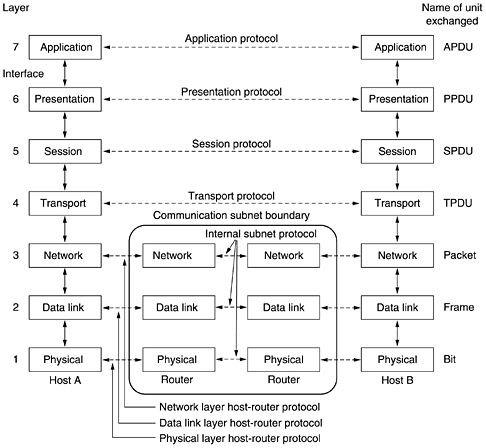
\includegraphics[width=\textwidth]{images/01fig20.png}
   \caption{The OSI Reference Model}
   \label{fig:osi-model}
\end{figure}


The OSI model has seven layers.
The principles that were applied to arrive at the seven layers can be briefly summarized as follows:

\begin{enumerate}
\item A layer should be created where a different abstraction is needed.
\item Each layer should perform a well-defined function.
\item The function of each layer should be chosen with an eye toward defining internationally standardized protocols.
\item The layer boundaries should be chosen to minimize the information flow across the interfaces.
\item The number of layers should be large enough that distinct functions need not be thrown together in the same layer out of necessity and small enough that the architecture does not become unwieldy.
\end{enumerate}

Below we will discuss each layer of the model in turn, starting at the
bottom layer. Note that the OSI model itself is not a network
architecture because it does not specify the exact services and
protocols to be used in each layer. It just tells what each layer should
do. However, ISO has also produced standards for all the layers,
although these are not part of the reference model itself. Each one has
been published as a separate international standard.

\subsubsection{The physical layer}

The \emph{physical layer} is concerned with transmitting raw bits over a communication channel.
The design issues have to do with making sure that when one side sends a 1 bit, it is received by the other side as a 1 bit, not as a 0 bit.
Typical questions here are how many volts should be used to represent a 1 and how many for a 0, how many nanoseconds a bit lasts, whether transmission may proceed simultaneously in both directions, how the initial connection is established and how it is torn down when both sides are finished, and how many pins the network connector has and what each pin is used for.
The design issues here largely deal with mechanical, electrical, and timing interfaces, and the physical transmission medium, which lies below the physical layer.


\subsubsection{The data link layer}

The main task of the \emph{data link layer} is to transform a raw transmission facility into a line that appears free of undetected
transmission errors to the network layer.
It accomplishes this task by having the sender break up the input data into \emph{data frames} (typically a few hundred or a few thousand bytes) and transmit the frames sequentially.
If the service is reliable, the receiver confirms correct receipt of each frame by sending back an \emph{acknowledgement frame}.

Another issue that arises in the data link layer (and most of the higher layers as well) is how to keep a fast transmitter from drowning a slow receiver in data.
Some traffic regulation mechanism is often needed to let the transmitter know how much buffer space the receiver has at the moment.
Frequently, this flow regulation and the error handling are integrated.

Broadcast networks have an additional issue in the data link layer: how to control access to the shared channel.
A special sublayer of the data link layer, the medium access control sublayer, deals with this problem.


\subsubsection{The network layer}

The \emph{network layer} controls the operation of the subnet.
A key design issue is determining how packets are routed from source to destination.
Routes can be based on static tables that are ``wired into'' the network and rarely changed.
They can also be determined at the start of each conversation, for example, a terminal session (e.g., a login to a remote
machine). Finally, they can be highly dynamic, being determined anew for
each packet, to reflect the current network load.

If too many packets are present in the subnet at the same time, they
will get in one another's way, forming bottlenecks. The control of such
congestion also belongs to the network layer. More generally, the
\emph{quality of service} provided (delay, transit time, jitter, etc.) is also a network layer issue.

When a packet has to travel from one network to another to get to its
destination, many problems can arise. The addressing used by the second
network may be different from the first one. The second one may not
accept the packet at all because it is too large. The protocols may
differ, and so on. It is up to the network layer to overcome all these
problems to allow heterogeneous networks to be interconnected.

In broadcast networks, the routing problem is simple, so the network
layer is often thin or even nonexistent.



\subsubsection{The transport layer}

The basic function of the \emph{transport layer} is to accept data from
above, split it up into smaller units if need be, pass these to the
network layer, and ensure that the pieces all arrive correctly at the
other end. Furthermore, all this must be done efficiently and in a way
that isolates the upper layers from the inevitable changes in the
hardware technology.

The transport layer also determines what type of service to provide to
the session layer, and, ultimately, to the users of the network. The
most popular type of transport connection is an error-free
point-to-point channel that delivers messages or bytes in the order in
which they were sent. However, other possible kinds of transport service
are the transporting of isolated messages, with no guarantee about the
order of delivery, and the broadcasting of messages to multiple
destinations. The type of service is determined when the connection is
established. (As an aside, an error-free channel is impossible to
achieve; what people really mean by this term is that the error rate is
low enough to ignore in practice.)

The transport layer is a true end-to-end layer, all the way from the
source to the destination. In other words, a program on the source
machine carries on a conversation with a similar program on the
destination machine, using the message headers and control messages. In
the lower layers, the protocols are between each machine and its
immediate neighbors, and not between the ultimate source and destination
machines, which may be separated by many routers. The difference between
layers 1 through 3, which are chained, and layers 4 through 7, which are
end-to-end, is illustrated in \vref{fig:osi-model}.


\subsubsection{The session layer}

The session layer allows users on different machines to establish
{sessions} between them. Sessions offer various services, including
{dialog control} (keeping track of whose turn it is to transmit), {token
management} (preventing two parties from attempting the same critical
operation at the same time), and {synchronization} (checkpointing long
transmissions to allow them to continue from where they were after a
crash).


\subsubsection{The presentation layer}

Unlike lower layers, which are mostly concerned with moving bits around,
the {presentation layer} is concerned with the syntax and semantics of
the information transmitted. In order to make it possible for computers
with different data representations to communicate, the data structures
to be exchanged can be defined in an abstract way, along with a standard
encoding to be used ``on the wire.''
The presentation layer manages these abstract data structures and allows higher-level data structures (e.g., banking records), to be defined and exchanged.


\subsubsection{The application layer}

The \emph{application layer} contains a variety of protocols that are commonly needed by users.
One widely-used application protocol is {HTTP} ({Hypertext Transfer Protocol}), which is the basis for the World Wide Web.
When a browser wants a Web page, it sends the name of the page it wants to the server using HTTP.
The server then sends the page back.
Other application protocols are used for file transfer, electronic mail, and network news.



\subsection{The TCP/IP Reference Model}

Let us now turn from the OSI reference model to the reference model used
in the grandparent of all wide area computer networks, the ARPANET, and
its successor, the worldwide Internet. Although we will give a brief
history of the ARPANET later, it is useful to mention a few key aspects
of it now. The ARPANET was a research network sponsored by the DoD (U.S.
Department of Defense). It eventually connected hundreds of universities
and government installations, using leased telephone lines. When
satellite and radio networks were added later, the existing protocols
had trouble interworking with them, so a new reference architecture was
needed. Thus, the ability to connect multiple networks in a seamless way
was one of the major design goals from the very beginning. This
architecture later became known as the {TCP/IP Reference Model}, after
its two primary protocols. It was first defined in (Cerf and Kahn,
1974). A later perspective is given in (Leiner et al., 1985). The design
philosophy behind the model is discussed in (Clark, 1988).

Given the DoD's worry that some of its precious hosts, routers, and
internetwork gateways might get blown to pieces at a moment's notice,
another major goal was that the network be able to survive loss of
subnet hardware, with existing conversations not being broken off. In
other words, DoD wanted connections to remain intact as long as the
source and destination machines were functioning, even if some of the
machines or transmission lines in between were suddenly put out of
operation. Furthermore, a flexible architecture was needed since
applications with divergent requirements were envisioned, ranging from
transferring files to real-time speech transmission.


\subsubsection{The internet layer}

All these requirements led to the choice of a packet-switching network
based on a connectionless internetwork layer. This layer, called the
\emph{internet layer}, is the linchpin that holds the whole architecture
together. Its job is to permit hosts to inject packets into any network
and have them travel independently to the destination (potentially on a
different network). They may even arrive in a different order than they
were sent, in which case it is the job of higher layers to rearrange
them, if in-order delivery is desired. Note that ``internet'' is used
here in a generic sense, even though this layer is present in the
Internet.

The analogy here is with the (snail) mail system. A person can drop a
sequence of international letters into a mail box in one country, and
with a little luck, most of them will be delivered to the correct
address in the destination country. Probably the letters will travel
through one or more international mail gateways along the way, but this
is transparent to the users. Furthermore, that each country (i.e., each
network) has its own stamps, preferred envelope sizes, and delivery
rules is hidden from the users.

The internet layer defines an official packet format and protocol called
{IP} ({Internet Protocol}). The job of the internet layer is to deliver
IP packets where they are supposed to go. Packet routing is clearly the
major issue here, as is avoiding congestion. For these reasons, it is
reasonable to say that the TCP/IP internet layer is similar in
functionality to the OSI network layer.
\Cref{fig:tcpip-model} shows this correspondence.


\begin{figure}
   \centering
   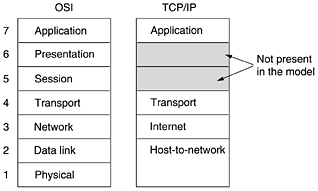
\includegraphics[width=.8\textwidth]{images/01fig21.png}
   \caption{The TCP/IP reference model}
   \label{fig:tcpip-model}
\end{figure}


\subsubsection{The transport layer}

The layer above the internet layer in the TCP/IP model is now usually
called the {transport layer}. It is designed to allow peer entities on
the source and destination hosts to carry on a conversation, just as in
the OSI transport layer. Two end-to-end transport protocols have been
defined here. The first one, {TCP} ({Transmission Control Protocol}), is
a reliable connection-oriented protocol that allows a byte stream
originating on one machine to be delivered without error on any other
machine in the internet. It fragments the incoming byte stream into
discrete messages and passes each one on to the internet layer. At the
destination, the receiving TCP process reassembles the received messages
into the output stream. TCP also handles flow control to make sure a
fast sender cannot swamp a slow receiver with more messages than it can
handle.

The second protocol in this layer, {UDP} ({User Datagram Protocol}), is
an unreliable, connectionless protocol for applications that do not want
TCP's sequencing or flow control and wish to provide their own. It is
also widely used for one-shot, client-server-type request-reply queries
and applications in which prompt delivery is more important than
accurate delivery, such as transmitting speech or video. The relation of
IP, TCP, and UDP is shown in \cref{fig:tcpip-model-protocols}.
Since the model was developed, IP has been implemented on many other networks.



\begin{figure}
   \centering
   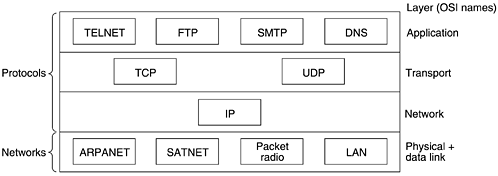
\includegraphics[width=\textwidth]{images/01fig22.png}
   \caption{Protocols and networks in the TCP/IP model initially}
   \label{fig:tcpip-model-protocols}
\end{figure}



\subsubsection{The application layer}

The TCP/IP model does not have session or presentation layers. No need
for them was perceived, so they were not included. Experience with the
OSI model has proven this view correct: they are of little use to most
applications.

On top of the transport layer is the \emph{application layer}.
It contains all the higher-level protocols.
The early ones included virtual terminal (TELNET), file transfer (FTP), and electronic mail (SMTP), as shown in \cref{fig:tcpip-model-protocols}.
The virtual terminal protocol allows a user on one machine to log onto a distant machine and work there.
The file transfer protocol provides a way to move data efficiently from one machine to another.
Electronic mail was originally just a kind of file transfer, but later a specialized protocol (SMTP) was developed for it.
Many other protocols have been added to these over the years: the Domain Name System (DNS) for mapping host names onto their network addresses, NNTP, the protocol for moving USENET news articles around, and HTTP, the protocol for fetching pages on the World Wide Web, and many others.


\subsubsection{The host-to-network layer}

Below the internet layer is a great void. The TCP/IP reference model
does not really say much about what happens here, except to point out
that the host has to connect to the network using some protocol so it
can send IP packets to it. This protocol is not defined and varies from
host to host and network to network. Books and papers about the TCP/IP
model rarely discuss it.



\subsection{A comparison of the OSI and TCP/IP reference models}

The OSI and TCP/IP reference models have much in common. Both are based
on the concept of a stack of independent protocols. Also, the
functionality of the layers is roughly similar. For example, in both
models the layers up through and including the transport layer are there
to provide an end-to-end, network-independent transport service to
processes wishing to communicate. These layers form the transport
provider. Again in both models, the layers above transport are
application-oriented users of the transport service.

Despite these fundamental similarities, the two models also have many
differences. In this section we will focus on the key differences
between the two reference models. It is important to note that we are
comparing the {reference models} here, not the corresponding {protocol
stacks}. The protocols themselves will be discussed later. For an entire
book comparing and contrasting TCP/IP and OSI, see (Piscitello and
Chapin, 1993).

Three concepts are central to the OSI model:
\begin{enumerate}
\item services,
\item interfaces, and
\item protocols.
\end{enumerate}

Probably the biggest contribution of the OSI model is to make the distinction between these three concepts explicit.
Each layer performs some services for the layer above it. The {service} definition tells what the layer does, not how entities above it access it or how the
layer works. It defines the layer's semantics.

A layer's {interface} tells the processes above it how to access it. It
specifies what the parameters are and what results to expect. It, too,
says nothing about how the layer works inside.

Finally, the peer {protocols} used in a layer are the layer's own
business. It can use any protocols it wants to, as long as it gets the
job done (i.e., provides the offered services). It can also change them
at will without affecting software in higher layers.

These ideas fit very nicely with modern ideas about object-oriented
programming. An object, like a layer, has a set of methods (operations)
that processes outside the object can invoke. The semantics of these
methods define the set of services that the object offers. The methods'
parameters and results form the object's interface. The code internal to
the object is its protocol and is not visible or of any concern outside
the object.

The TCP/IP model did not originally clearly distinguish between service,
interface, and protocol, although people have tried to retrofit it after
the fact to make it more OSI-like. For example, the only real services
offered by the internet layer are SEND IP PACKET and RECEIVE IP PACKET.

As a consequence, the protocols in the OSI model are better hidden than
in the TCP/IP model and can be replaced relatively easily as the
technology changes. Being able to make such changes is one of the main
purposes of having layered protocols in the first place.

The OSI reference model was devised {before} the corresponding protocols
were invented. This ordering means that the model was not biased toward
one particular set of protocols, a fact that made it quite general. The
downside of this ordering is that the designers did not have much
experience with the subject and did not have a good idea of which
functionality to put in which layer.

For example, the data link layer originally dealt only with
point-to-point networks. When broadcast networks came around, a new
sublayer had to be hacked into the model. When people started to build
real networks using the OSI model and existing protocols, it was
discovered that these networks did not match the required service
specifications (wonder of wonders), so convergence sublayers had to be
grafted onto the model to provide a place for papering over the
differences. Finally, the committee originally expected that each
country would have one network, run by the government and using the OSI
protocols, so no thought was given to internetworking. To make a long
story short, things did not turn out that way.

With TCP/IP the reverse was true: the protocols came first, and the
model was really just a description of the existing protocols. There was
no problem with the protocols fitting the model. They fit perfectly. The
only trouble was that the {model} did not fit any other protocol stacks.
Consequently, it was not especially useful for describing other,
non-TCP/IP networks.

Turning from philosophical matters to more specific ones, an obvious
difference between the two models is the number of layers: the OSI model
has seven layers and the TCP/IP has four layers. Both have
(inter)network, transport, and application layers, but the other layers
are different.

Another difference is in the area of connectionless versus
connection-oriented communication. The OSI model supports both
connectionless and connection-oriented communication in the network
layer, but only connection-oriented communication in the transport
layer, where it counts (because the transport service is visible to the
users). The TCP/IP model has only one mode in the network layer
(connectionless) but supports both modes in the transport layer, giving
the users a choice. This choice is especially important for simple
request-response protocols.


\subsection{A critique of the OSI model and protocols}

Neither the OSI model and its protocols nor the TCP/IP model and its
protocols are perfect. Quite a bit of criticism can be, and has been,
directed at both of them. In this section and the next one, we will look
at some of these criticisms. We will begin with OSI and examine TCP/IP
afterward.

At the time the second edition of this book was published (1989), it
appeared to many experts in the field that the OSI model and its
protocols were going to take over the world and push everything else out
of their way. This did not happen. Why? A look back at some of the
lessons may be useful. These lessons can be summarized as:

\begin{enumerate}
\item Bad timing.
\item Bad technology.
\item Bad implementations.
\item Bad politics.
\end{enumerate}


\subsubsection{Bad timing}

First let us look at reason one: bad timing. The time at which a standard is established is absolutely critical to its success.
David Clark of MIT\ has a theory of standards that he calls the {apocalypse of the two elephants}, which is illustrated in \cref{fig:two-elephants}.

\begin{figure}
   \centering
   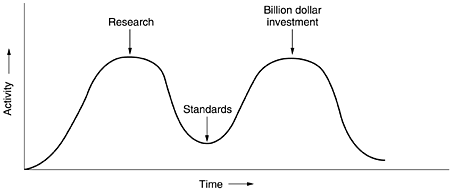
\includegraphics[width=\textwidth]{images/01fig23.png}
   \caption{The apocalypse of the two elephants}
   \label{fig:two-elephants}
\end{figure}


This figure shows the amount of activity surrounding a new subject. When
the subject is first discovered, there is a burst of research activity
in the form of discussions, papers, and meetings. After a while this
activity subsides, corporations discover the subject, and the
billion-dollar wave of investment hits.

It is essential that the standards be written in the trough in between
the two ``elephants.''
If the standards are written too early, before
the research is finished, the subject may still be poorly understood;
the result is bad standards. If they are written too late, so many
companies may have already made major investments in different ways of
doing things that the standards are effectively ignored. If the interval
between the two elephants is very short (because everyone is in a hurry
to get started), the people developing the standards may get crushed.

It now appears that the standard OSI protocols got crushed. The
competing TCP/IP protocols were already in widespread use by research
universities by the time the OSI protocols appeared. While the
billion-dollar wave of investment had not yet hit, the academic market
was large enough that many vendors had begun cautiously offering TCP/IP
products. When OSI came around, they did not want to support a second
protocol stack until they were forced to, so there were no initial
offerings. With every company waiting for every other company to go
first, no company went first and OSI never happened.


\subsubsection{Bad technology}

The second reason that OSI never caught on is that both the model and
the protocols are flawed. The choice of seven layers was more political
than technical, and two of the layers (session and presentation) are
nearly empty, whereas two other ones (data link and network) are
overfull.

The OSI model, along with the associated service definitions and protocols, is extraordinarily complex.
When piled up, the printed standards occupy a significant fraction of a meter of paper.
They are also difficult to implement and inefficient in operation.
In this context, a riddle posed by Paul Mockapetris and cited in (Rose, 1993) comes to mind:

\begin{quote}
   \textbf{Question:}
   What do you get when you cross a mobster with an international standard?\\
   \textbf{Answer:}
   Someone who makes you an offer you can't understand.
\end{quote}

In addition to being incomprehensible, another problem with OSI is that
some functions, such as addressing, flow control, and error control,
reappear again and again in each layer. Saltzer et al. (1984), for
example, have pointed out that to be effective, error control must be
done in the highest layer, so that repeating it over and over in each of
the lower layers is often unnecessary and inefficient.



\subsubsection{Bad implementations}

Given the enormous complexity of the model and the protocols, it will
come as no surprise that the initial implementations were huge,
unwieldy, and slow. Everyone who tried them got burned. It did not take
long for people to associate ``OSI'' with ``poor quality.''
Although the products improved in the course of time, the image stuck.

In contrast, one of the first implementations of TCP/IP was part of
Berkeley UNIX and was quite good (not to mention, free). People began
using it quickly, which led to a large user community, which led to
improvements, which led to an even larger community. Here the spiral was
upward instead of downward.


\subsubsection{Bad politics}

On account of the initial implementation, many people, especially in
academia, thought of TCP/IP as part of UNIX, and UNIX in the 1980s in
academia was not unlike parenthood (then incorrectly called motherhood)
and apple pie.

OSI, on the other hand, was widely thought to be the creature of the
European telecommunication ministries, the European Community, and later
the U.S. Government. This belief was only partly true, but the very idea
of a bunch of government bureaucrats trying to shove a technically
inferior standard down the throats of the poor researchers and
programmers down in the trenches actually developing computer networks
did not help much. Some people viewed this development in the same light
as IBM announcing in the 1960s that PL/I was the language of the future,
or DoD correcting this later by announcing that it was actually Ada.



\subsection{A critique of the TCP/IP reference model}

The TCP/IP model and protocols have their problems too.
First, the model does not clearly distinguish the concepts of service, interface, and
protocol. Good software engineering practice requires differentiating
between the specification and the implementation, something that OSI
does very carefully, and TCP/IP does not. Consequently, the TCP/IP model
is not much of a guide for designing new networks using new
technologies.

Second, the TCP/IP model is not at all general and is poorly suited to
describing any protocol stack other than TCP/IP. Trying to use the
TCP/IP model to describe Bluetooth, for example, is completely
impossible.

Third, the host-to-network layer is not really a layer at all in the
normal sense of the term as used in the context of layered protocols. It
is an interface (between the network and data link layers). The
distinction between an interface and a layer is crucial, and one should
not be sloppy about it.

Fourth, the TCP/IP model does not distinguish (or even mention) the
physical and data link layers. These are completely different. The
physical layer has to do with the transmission characteristics of copper
wire, fiber optics, and wireless communication. The data link layer's
job is to delimit the start and end of frames and get them from one side
to the other with the desired degree of reliability. A proper model
should include both as separate layers. The TCP/IP model does not do
this.

Finally, although the IP and TCP protocols were carefully thought out
and well implemented, many of the other protocols were ad hoc, generally
produced by a couple of graduate students hacking away until they got
tired. The protocol implementations were then distributed free, which
resulted in their becoming widely used, deeply entrenched, and thus hard
to replace. Some of them are a bit of an embarrassment now. The virtual
terminal protocol, TELNET, for example, was designed for a ten-character
per second mechanical Teletype terminal. It knows nothing of graphical
user interfaces and mice. Nevertheless, 25 years later, it is still in
widespread use.

In summary, despite its problems, the OSI {model} (minus the session and
presentation layers) has proven to be exceptionally useful for
discussing computer networks. In contrast, the OSI {protocols} have not
become popular. The reverse is true of TCP/IP: the {model} is
practically nonexistent, but the {protocols} are widely used. Since
computer scientists like to have their cake and eat it, too, in this
book we will use a modified OSI model but concentrate primarily on the
TCP/IP and related protocols, as well as newer ones such as 802, SONET,
and Bluetooth.
In effect, we will use the hybrid model of \cref{fig:hybrid-model}.


\begin{figure}
   \centering
   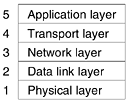
\includegraphics[width=.2\textwidth]{images/01fig24.png}
   \caption{The hybrid reference model to be used in this book.}
   \label{fig:hybrid-model}
\end{figure}

